\documentclass{article}
\usepackage[T1]{fontenc}
\usepackage{lmodern}
\usepackage[polish]{babel}
\usepackage{graphicx}
\usepackage{float}
\usepackage{hyperref}

\usepackage[a4paper, margin=2.54cm]{geometry}

\title{Raport skuteczności wybranych modeli}
\author{Maciej Szefler, Kacper Karski,
    \\Damian Jankowski, Filip Krawczak}

\begin{document}

\maketitle

\tableofcontents

\section{Las losowy}
\subsection{Wstęp}

Las Losowy (ang. Random Forest) to algorytm uczenia maszynowego, który jest używany zarówno do zadań klasyfikacji, jak i regresji. Jest to przykład metody która polega na łączeniu wyników wielu modeli bazowych w celu uzyskania lepszej ogólnej wydajności. Działanie tego algorytmu polega na losowym wyborze podzbiorów danych z zestawu treningowego. Każde drzewo jest trenowane na innym podzbiorze danych, co wprowadza losowość i różnorodność w procesie uczenia. Podczas budowy każdego drzewa, losowo wybiera się tylko pewną liczbę cech spośród wszystkich dostępnych cech. Ten proces pomaga w zwiększeniu różnorodności modeli i unika przewagi nadmiernie wpływających cech. Następnie w przypadku klasyfikacji, algorytm Lasu Losowego przewiduje wynik na podstawie głosowania drzew, wybierając najczęściej występującą klasę. W przypadku regresji, przewiduje się średnią wartość przewidywaną przez wszystkie drzewa. Dzięki losowym podzbiorom danych i cech oraz kombinacji wielu drzew, Las Losowy jest generalnie mniej podatny na przeuczenie (ang. overfitting) niż pojedyncze drzewo decyzyjne. Różnorodność drzew pomaga w zwiększeniu ogólnej zdolności do generalizacji modelu.  Przewagą algorytmu lasu losowego jest jego wysoka skuteczność w stosunku do relatywnie niskiej ilości próbek.

Wykorzystany algorytm lasu losowego klasyfikuje znormalizowane dane związane z oddechem. Algorytm jest używany do przewidywania trzech stanów: bezdech, wdech i wydech, na podstawie otrzymanych 5 próbek, dla których określa stan oddechu. Sklasyfikowane dane następnie są przekazywane jako dane treningowe do modelu sieci neuronowej. Cały proces można określić jako uproszczony Transfer Labelling. Algorytm Lasu Losowego działa jako etap wstępny do etapu uczenia sieci neuronowej, co prowadzi do lepszych wyników klasyfikacji danych związanych z oddechem.


\subsection{Wyniki}

\begin{figure}[H]
    \centering
    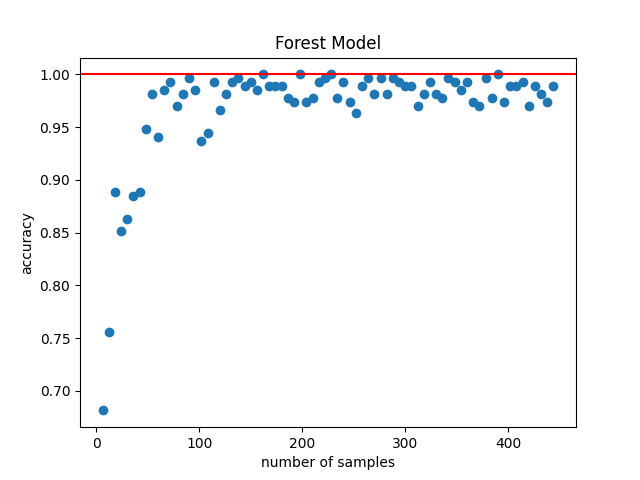
\includegraphics[width=0.75\textwidth]{las_losowy/transfer_labelling_forest.png}
    \caption{Skuteczność lasu losowego w zależności od liczby próbek treningowych}
    \label{fig:data_chart1}
\end{figure}

Rys. \ref{fig:data_chart1} przedstawia zależność między liczbą próbek a dokładnością modelu lasów losowych. Punkty na wykresie reprezentują dokładność modelu dla różnych liczb próbek użytych do treningu. Linia pozioma wskazuje na wartość dokładności równej 1.00, która jest teoretycznym maksimum.

Na podstawie rozproszenia punktów można zaobserwować, że dokładność modelu generalnie wzrasta wraz z liczebnością próbek, osiągając stabilizację blisko maksymalnej możliwej wartości dokładności. Większość punktów koncentruje się w górnej części wykresu, powyżej wartości dokładności 0.95, co wskazuje na wysoką wydajność modelu.

Jednakże, istnieje kilka punktów, które odstają od ogólnej tendencji, gdzie dokładność jest znacząco niższa, szczególnie przy mniejszej liczbie próbek. Te anomalie mogą wskazywać na przypadki, w których model miał trudności z generalizacją na skutek ograniczonej ilości danych lub specyficznych cech danych treningowych.

Podsumowując, przedstawione dane sugerują, że model lasów losowych osiąga wysoką dokładność w zadaniu klasyfikacyjnym, przy czym efektywność ta stabilizuje się przy większej liczbie próbek. Odstające wartości w dolnej części wykresu, mimo że są w mniejszości, mogą wymagać dodatkowej analizy, aby zrozumieć przyczyny niższej dokładności w tych przypadkach. Wyniki te wskazują na potencjalną potrzebę dalszej optymalizacji procesu treningowego lub przeglądu metody selekcji i przetwarzania próbek treningowych.
\newpage

W celu efektywnego wytrenowania modelu sieci neuronowych, pobrany został surowy sygnał z tensometru. Nie był na nim użyty żaden filtr, ani normalizacja. Dane surowe charakteryzują się dużymi wartościami m.in w zakresie 700 000 - 1 000 000 w zależności od wielkosści przepony osoby badanej. 

Przykładowy wygląd takich danych można zobaczyć na rys. \ref{fig:data_chart3} i \ref{fig:data_chart4}. Dane zostały podzielone na 3 grupy: wdech, wydech i bezdech i znoralizowane do zakresu (-1, 1) aby model był przystosowany do postury wszystkich badanych. Każda grupa zawierała 5 pomiarów które zostały przekształcone do postaci wektora o długości 6. Ostatnią wartością w wektorze była amplituda wszystkich 5 sygnałów. 

Tak przygotowane wektory zostały przekazane do pliku tekstowego, a na końcu każdego wektora, została dopisana wartość oznaczająca kategorię próbek (-1 jako wydech, 0 jako bezdech, 1 jako wdech). Tak przygotowany plik tekstowy został przekazany do modelu lasu losowego. Na podstawie tych danych, model został wytrenowany i zapisany do pliku.

\begin{figure}[H]
    \centering
    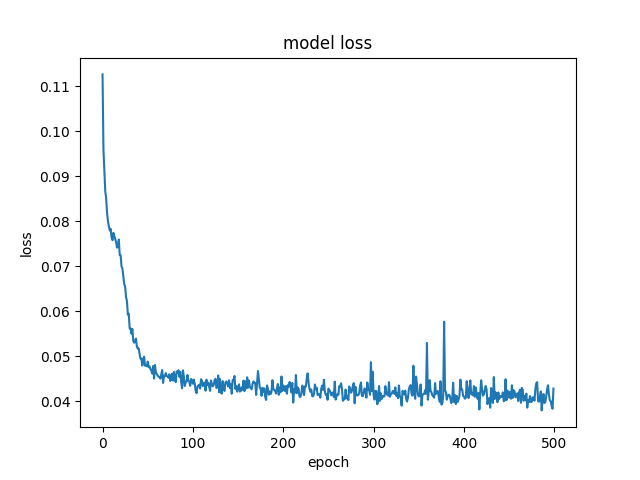
\includegraphics[width=0.75\textwidth]{las_losowy/epoch_loss_forest.png}
    \caption{Krzywa strat modelu lasów losowych}
    \label{fig:data_chart2}
\end{figure}

Rys. \ref{fig:data_chart2} przedstawia zmianę funkcji straty modelu sieci neuronowej w zależności od liczby epok w procesie uczenia. Widać, że wartość straty modelu gwałtownie spada w początkowej fazie uczenia, co wskazuje na szybką adaptację modelu do danych treningowych. Początkowa wartość straty znajduje się na poziomie około 0.11 i spada do około 0.05 już po niewielkiej liczbie epok.

Po tej wstępnej fazie, krzywa strat wykazuje trend spadkowy, osiągając stabilizację z niewielkimi fluktuacjami wokół wartości 0.04. Pojawienie się tych fluktuacji może sugerować momenty, w których model napotykał na trudniejsze do nauki przypadki w danych lub kiedy dostosowywał się do subtelniejszych cech danych treningowych.

Na wykresie obserwujemy także pewne artefakty w wartościach strat, które występują sporadycznie po około 400 epokach. Te artefakty mogą wskazywać na przeuczenie się modelu lub na niestabilności w procesie uczenia, co mogłoby być wynikiem na przykład zbyt wysokiej stopy uczenia się lub anomalii w danych treningowych.

Podsumowując, przedstawiony wykres pokazuje typową krzywą uczenia się dla modelu maszynowego, z szybkim postępem na początku i stabilizacją w miarę zbliżania się do optymalnej wydajności. Stabilizacja wartości straty na niskim poziomie wskazuje na to, że model osiągnął zadowalający poziom generalizacji. Jednakże, obserwowane fluktuacje i artefakty mogą wymagać dalszej analizy w celu zapewnienia, że model jest dobrze dostrojony i nie występuje przeuczenie.

\begin{figure}[H]
    \centering
    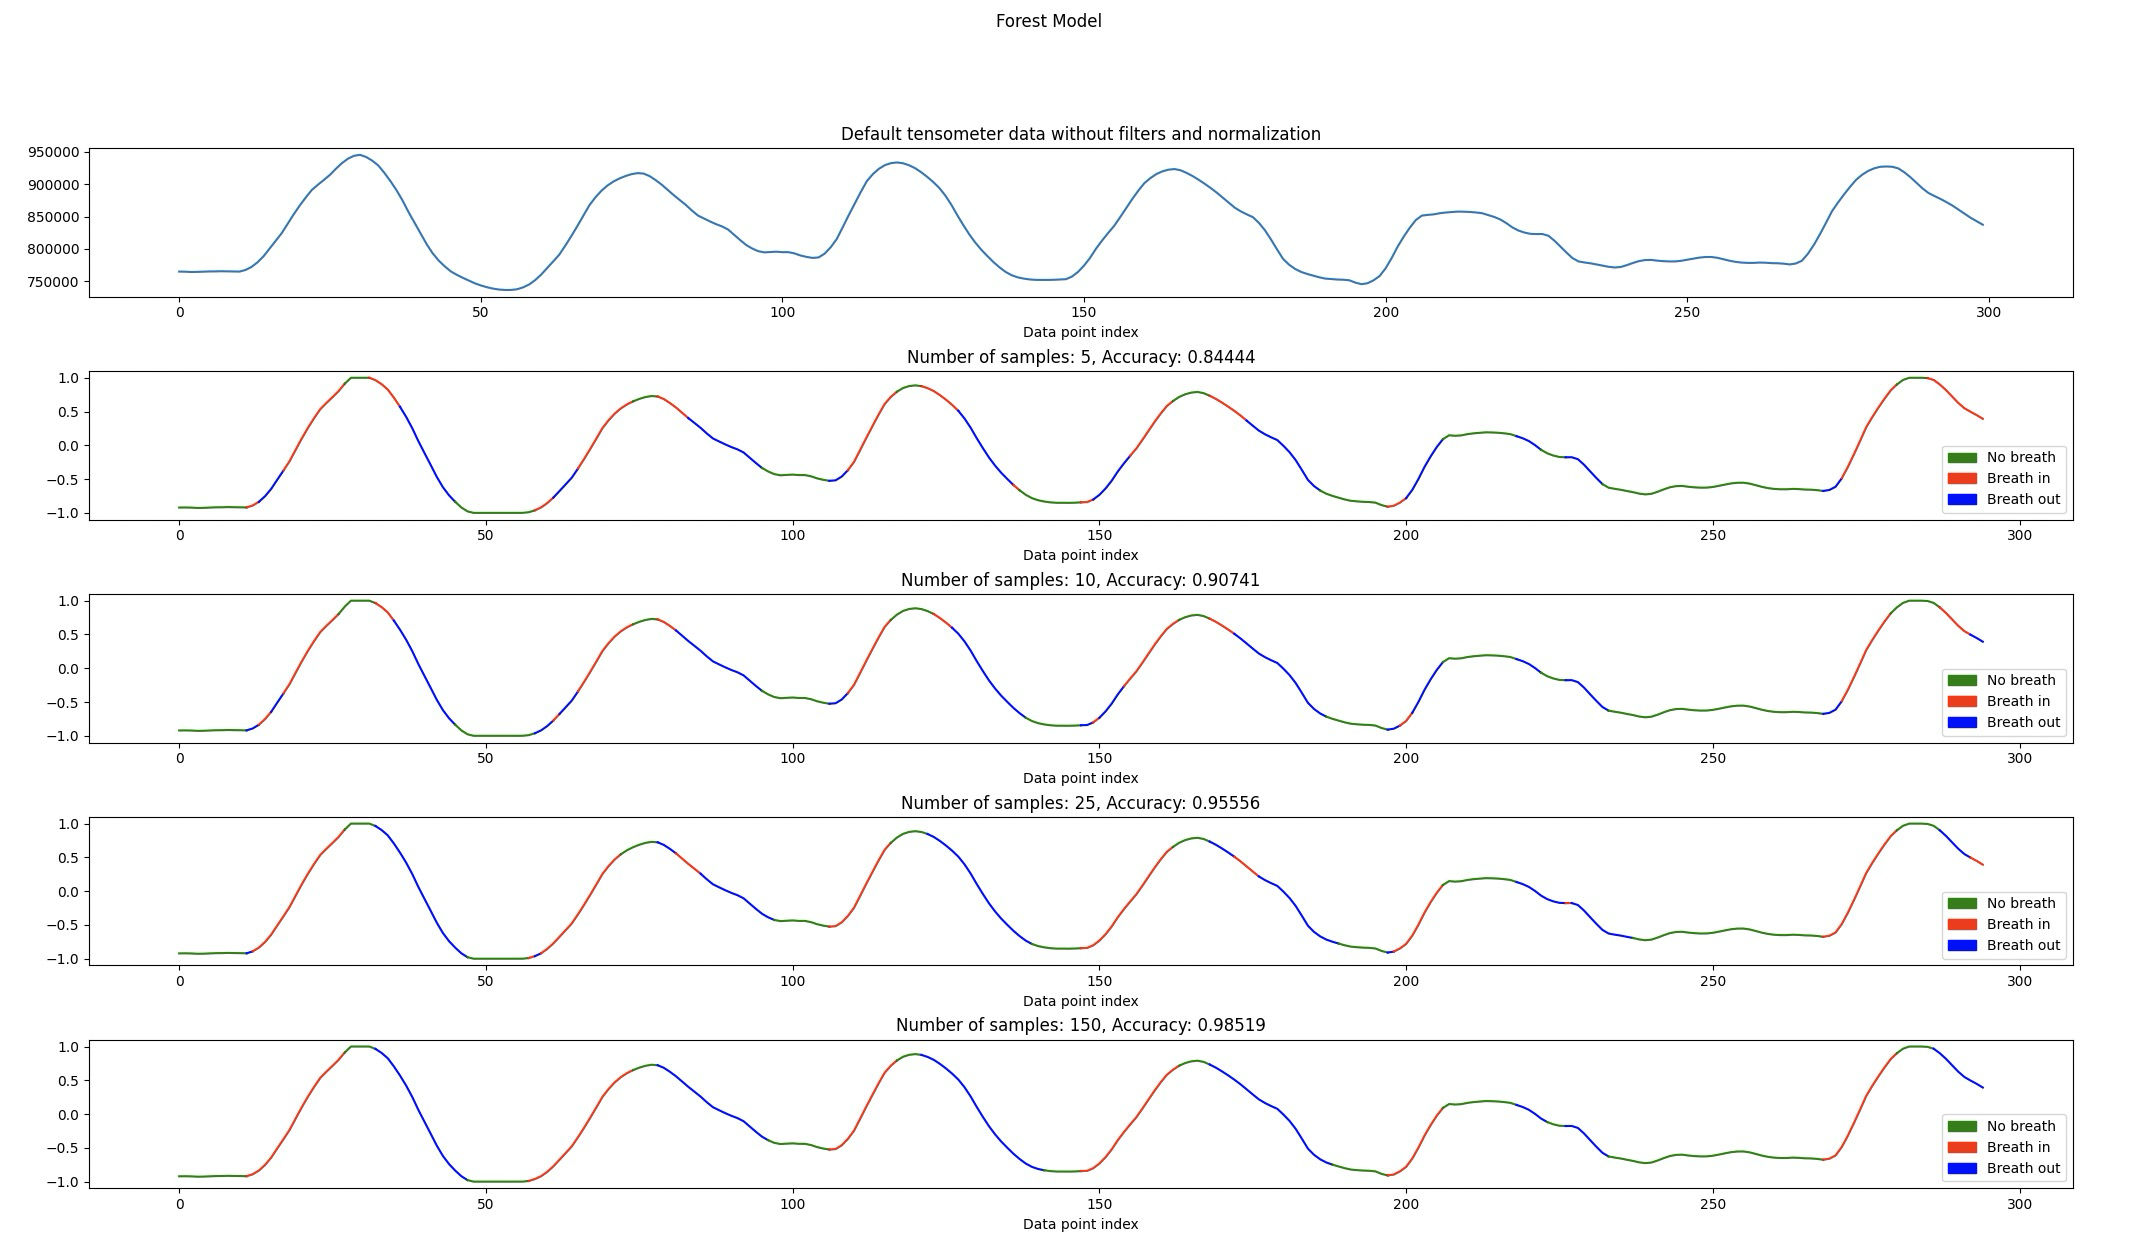
\includegraphics[width=\textwidth]{las_losowy/jak_sobie_radzi_las_losowy.png}
    \caption{Skuteczność lasu losowego od liczby próbek treningowych dla 300 próbek testowych}
    \label{fig:data_chart3}
\end{figure}

\begin{figure}[H]
    \centering
    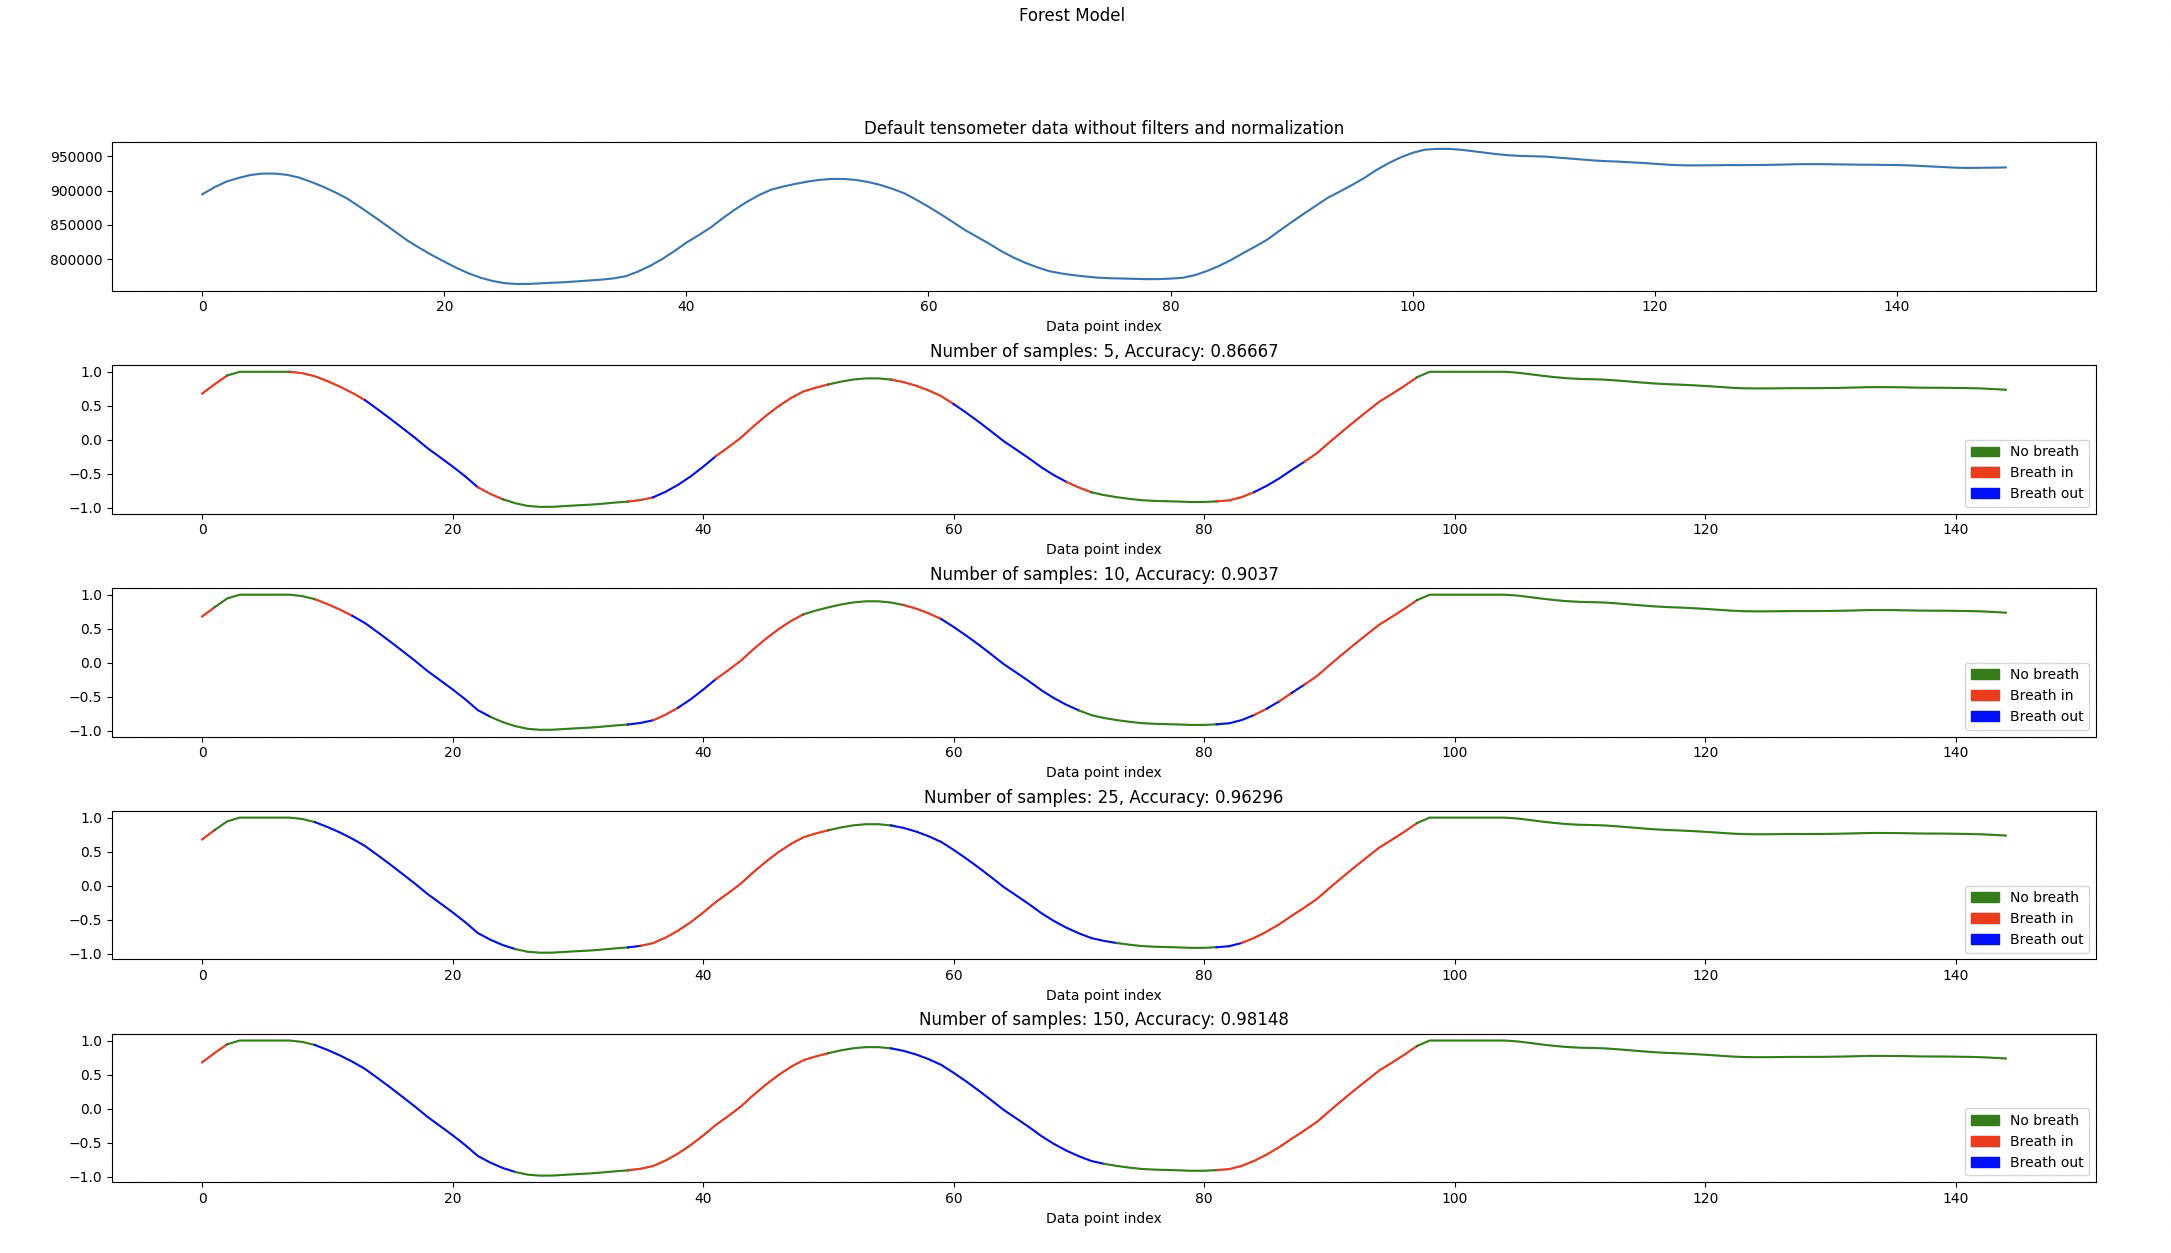
\includegraphics[width=\textwidth]{las_losowy/jak_sobie_radzi_las_losowy_2.png}
    \caption{Skuteczność lasu losowego od liczby próbek treningowych dla 150 próbek testowych}
    \label{fig:data_chart4}
\end{figure}

Przedstawione rys. \ref{fig:data_chart3} i \ref{fig:data_chart4} ilustrują efektywność modelu w zależności od liczby próbek wykorzystanych do treningu. Rys. \ref{fig:data_chart3} w sekwencji nie zawiera danych klasyfikacyjnych, służąc jako odniesienie do zestawu danych wejściowych bez zastosowania filtrów i normalizacji. Dane użyte do zaprezentowania wyników, przedstawiają standardowy oddech badanego. Nie zawierają one żadnych anomalii, takich jak np. kaszel, hiperwentylacja, wolny oddech, który mógłby wpłynąć na wyniki klasyfikacji. W daleszej cześci raportu, zostaną przedstawione ww. anomalie. Dokładność klasyfikacji jest obliczana na podstawie porównania przewidywanych etykiet (klas) przez model z rzeczywistymi etykietami w zbiorze testowym. W przypadku problemów klasyfikacyjnych, gdzie etykiety są liczbami całkowitymi reprezentującymi klasy, dokładność jest obliczona jako stosunek liczby poprawnych przewidywań do ogólnej liczby przykładów. Przykładowo dla danego eksperymentu, w którym liczba próbek wynosi 100, jeżeli poprawnie sklasyfikowano 85 próbek, dokładność wynosi 0.85.


W kolejnych eksperymentach, gdzie liczba próbek wykorzystanych do treningu wynosi odpowiednio 5, 10, 25 i 150 (ilość próbek dla każdego stanu), obserwujemy progresywną poprawę dokładności klasyfikacji od wartości $\sim$0.85 do $\sim$0.985. Wzrost dokładności jest korelowany z zwiększającą się liczbą próbek treningowych, co jest zgodne z powszechnie akceptowanymi założeniami w dziedzinie uczenia maszynowego. Dane te sugerują, że model Lasu Losowego wykazuje zdolność do generalizacji i poprawy wyników przy większej objętości danych treningowych.

Analizując przedstawione wykresy, można zauważyć że modele uczone na mniejszej liczbie próbek, słabo radzą sobie w momentach zaszumienia sygnałów. Szczególnie warto zwrócić uwagę na momenty zmian stanów. W takich sytuacjach, modele uczone na mniejszej liczbie próbek, niepoprawnie klasyfikują dane.

Rezultaty te mogą mieć znaczące implikacje dla monitorowania parametrów życiowych w realnym czasie, szczególnie w kontekście detekcji i analizy oddechu. Wysoka dokładność modelu przy wyższej liczbie próbek treningowych wskazuje na jego potencjalną przydatność w zastosowaniach klinicznych oraz w systemach wspierających decyzje medyczne.

\subsection{Anomalie}

\begin{figure}[H]
    \centering
    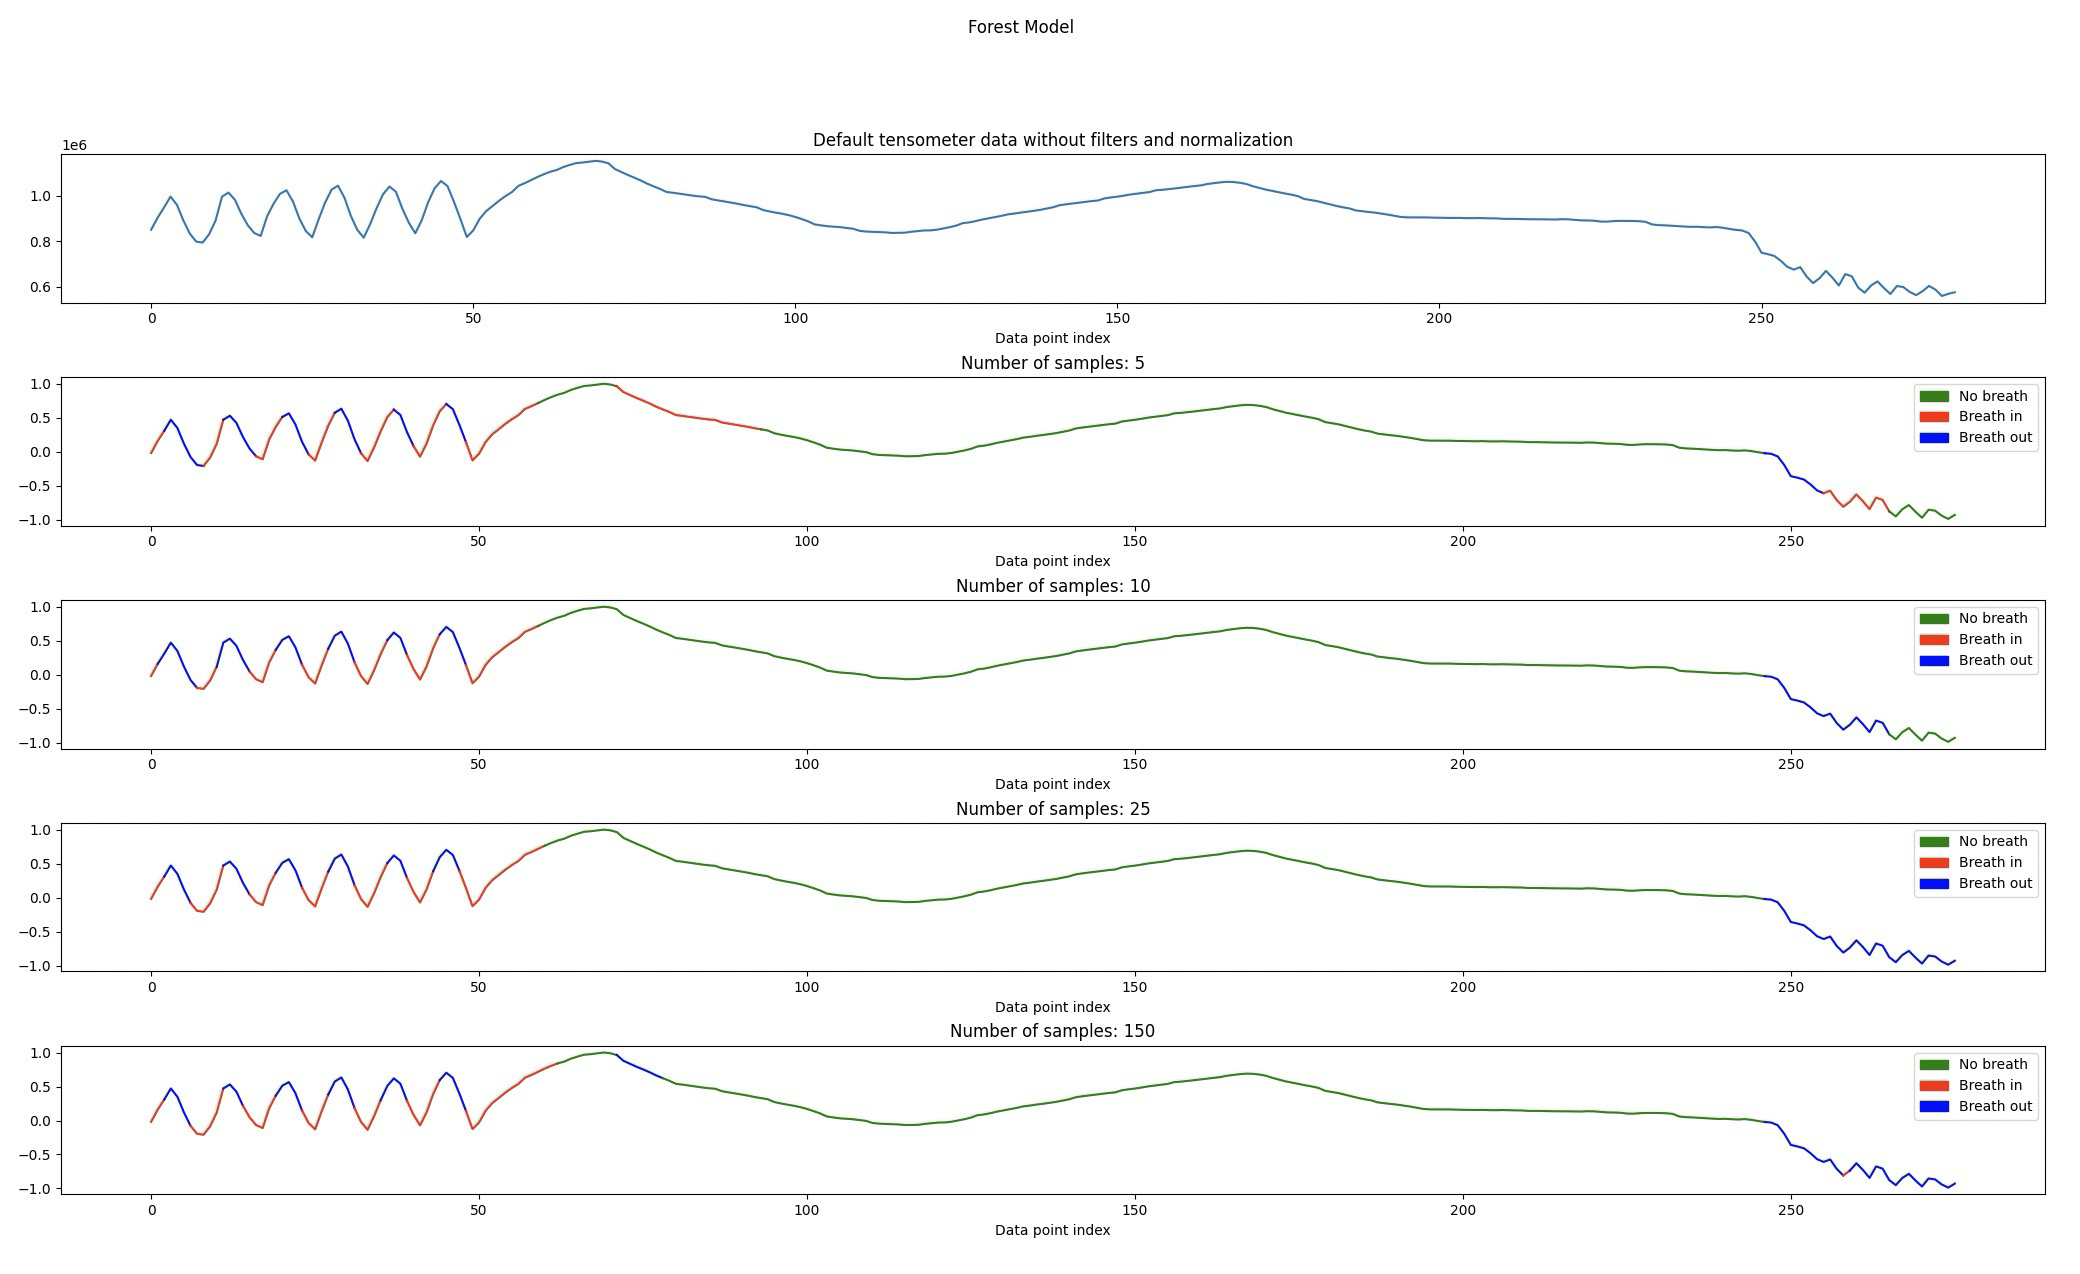
\includegraphics[width=\textwidth]{las_losowy/anomalie.png}
    \caption{Dane z anomaliami takimi jak hiperwentylacja, kaszel, wolny oddech}
    \label{fig:data_chart5}
\end{figure}

Przedstawiony rys. \ref{fig:data_chart5} ilustruje zdolność klasyfikacji modelu w przypadku danych z anomaliami. Dane te zawierają anomalie takie jak hiperwentylacja, wolny oddech i kaszel. Analizę warto rozpocząć od pierwszych 50 próbek które przedstawiają hiperwentylację. 

W tym przypadku model powinien oznaczyć początek hiperwentylacji jako wdech, a koniec jako wydech. W rzeczywistości, model oznacza zmiany stanu z wydechu na bezdech jako wdech, a zmianę z wdechu na wydech jako wydech. 

Kolejne 200 próbek dotyczy wolnego oddechu. W tym przypadku, model oznacza całość jako bezdech, chociaż powinien wykrywać zmiany stanu. 

W przypadku kaszlu, czyli ostatnik 50 próbek, model oznacza calość jako wydech. Jest to bardzo nienaturalny rytm oddechu i może stanowić swojego rodzaju artefakty. Takie przypadki są ciężkie do poprawnego sklasyfikowania, ze względu na bardzo duże szumy w krótkim odstępie czasu.

Żaden z powyższych przypadków nie został poprawnie sklasyfikowany przez model. Do uzyskania poprawnej klasyfikacji, model potrzebuje więcej próbek treningowych, które zawierają anomalie. Wynika to również z tego, że anomalie te są bardzo rzadkie i trudne do poprawnego sklasyfikowania, a w zbiorze na którym był trenowany las losowy, nie występowały powyższe przypadki. Aby poprawić działanie modelu, należy stworzyć osobne zbiory danych zawierające anomalie oraz ręcznie je oznaczyć. Tak przygotowane dane, pozwolą na poprawne działanie modelu w przypadku wystąpienia anomalii.

\section{Batch normalization model}

\subsection{Wstęp}

Batch Normalization (BN) to technika stosowana w głębokich sieciach neuronowych, która ma na celu poprawę procesu uczenia się poprzez normalizację aktywacji wewnątrz warstw. Działanie tego modelu polega na podziale zestawu danych treningowych na mniejsze paczki danych, a następnie normalizacje aktywacji poprzez odejmowanie średniej i dzielenie przez odchylenie standardowe mniejszej paczki danych (mini-batch). Po znormalizowaniu, dane są skalowane i przesuwane przy użyciu dwóch parametrów gamma i beta. Wartości te są parametrami trenowanymi podczas uczenia i pozwalają na elastyczną transformację danych. BN działa jak pewnego rodzaju regularyzacja poprzez wprowadzenie szumu do procesu treningu. To zjawisko zapobiega zbytniemu dostosowaniu się modelu do konkretnych danych treningowych. Podsumowując Batch Normalization przyspiesza uczenie - pozwala przy mniejszej liczbie iteracji uzyskać takie same rezultaty jak sieci nieposiadające tej normalizacji. Umożliwia zastosowanie wyższych learning rates bez negatywnych rezultatów oraz pomaga również eliminować overfitting.

\subsection{Wyniki}

\begin{figure}[H]
    \centering
    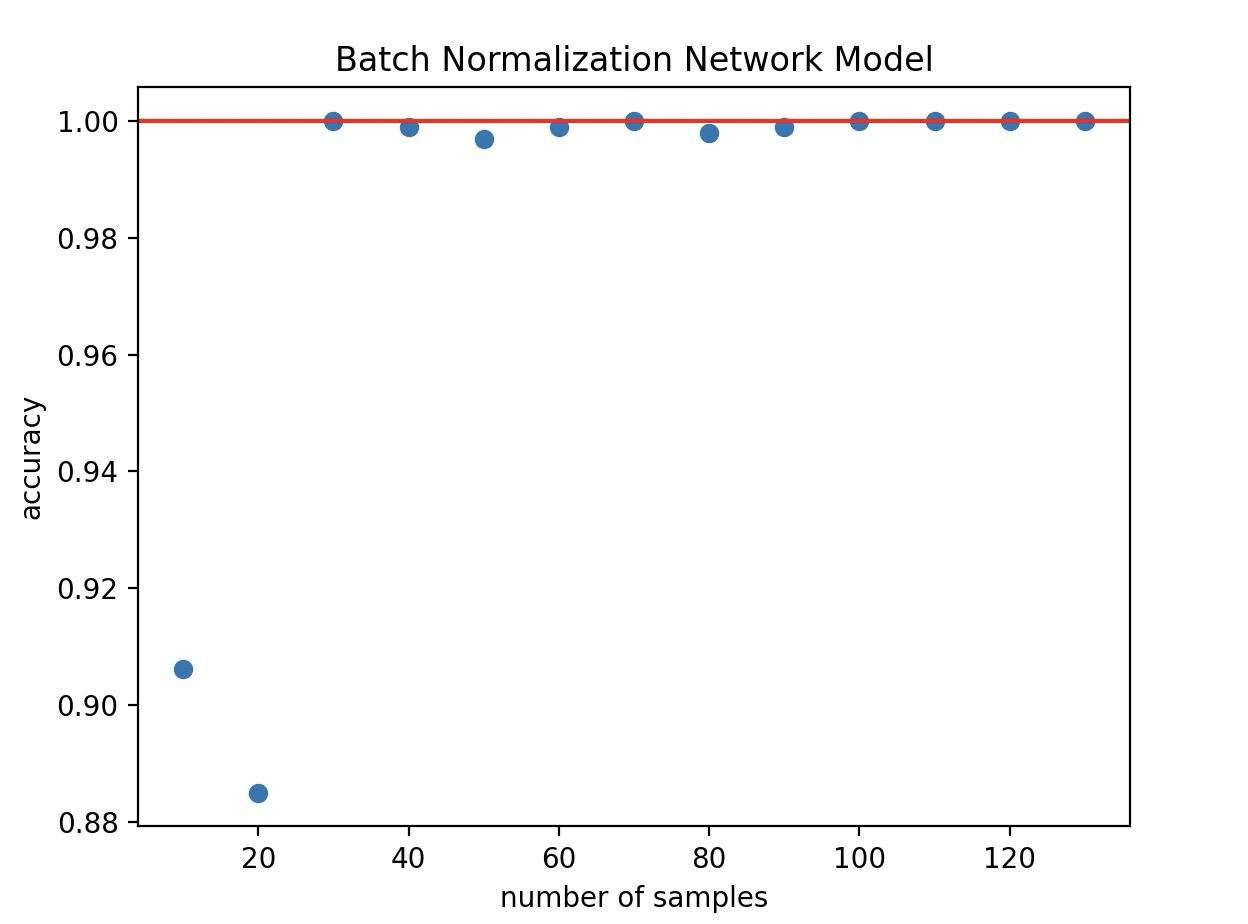
\includegraphics[width=0.75\textwidth]{batch_normalization/dokladnosc.png}
    \caption{Skuteczność modelu z Batch Normalization w zależności od liczby próbek treningowych}
    \label{fig:data_chart6}
\end{figure}

Rys. \ref{fig:data_chart6} przedstawia skuteczność modelu z Batch Normalization w zależności od liczby próbek treningowych. Punkty na wykresie reprezentują dokładność modelu dla różnych liczb próbek użytych do treningu. Linia pozioma wskazuje na wartość dokładności równej 1.00, która jest teoretycznym maksimum. Na podstawie rozproszenia punktów można zaobserwować, że dokładność modelu generalnie wzrasta wraz z liczebnością próbek, osiągając stabilizację blisko maksymalnej możliwej wartości dokładności. Większość punktów koncentruje się w górnej części wykresu, powyżej wartości dokładności 0.99, co wskazuje na wysoką wydajność modelu. Jednakże, istnieje kilka punktów, które odstają od ogólnej tendencji, gdzie dokładność jest znacząco niższa, szczególnie przy mniejszej liczbie próbek. Te anomalie mogą wskazywać na przypadki, w których model miał trudności z generalizacją na skutek ograniczonej ilości danych lub specyficznych cech danych treningowych. Podsumowując, przedstawione dane sugerują, że model z Batch Normalization osiąga wysoką dokładność w zadaniu klasyfikacyjnym, przy czym efektywność ta stabilizuje się przy większej liczbie próbek.

\begin{figure}[H]
    \centering
    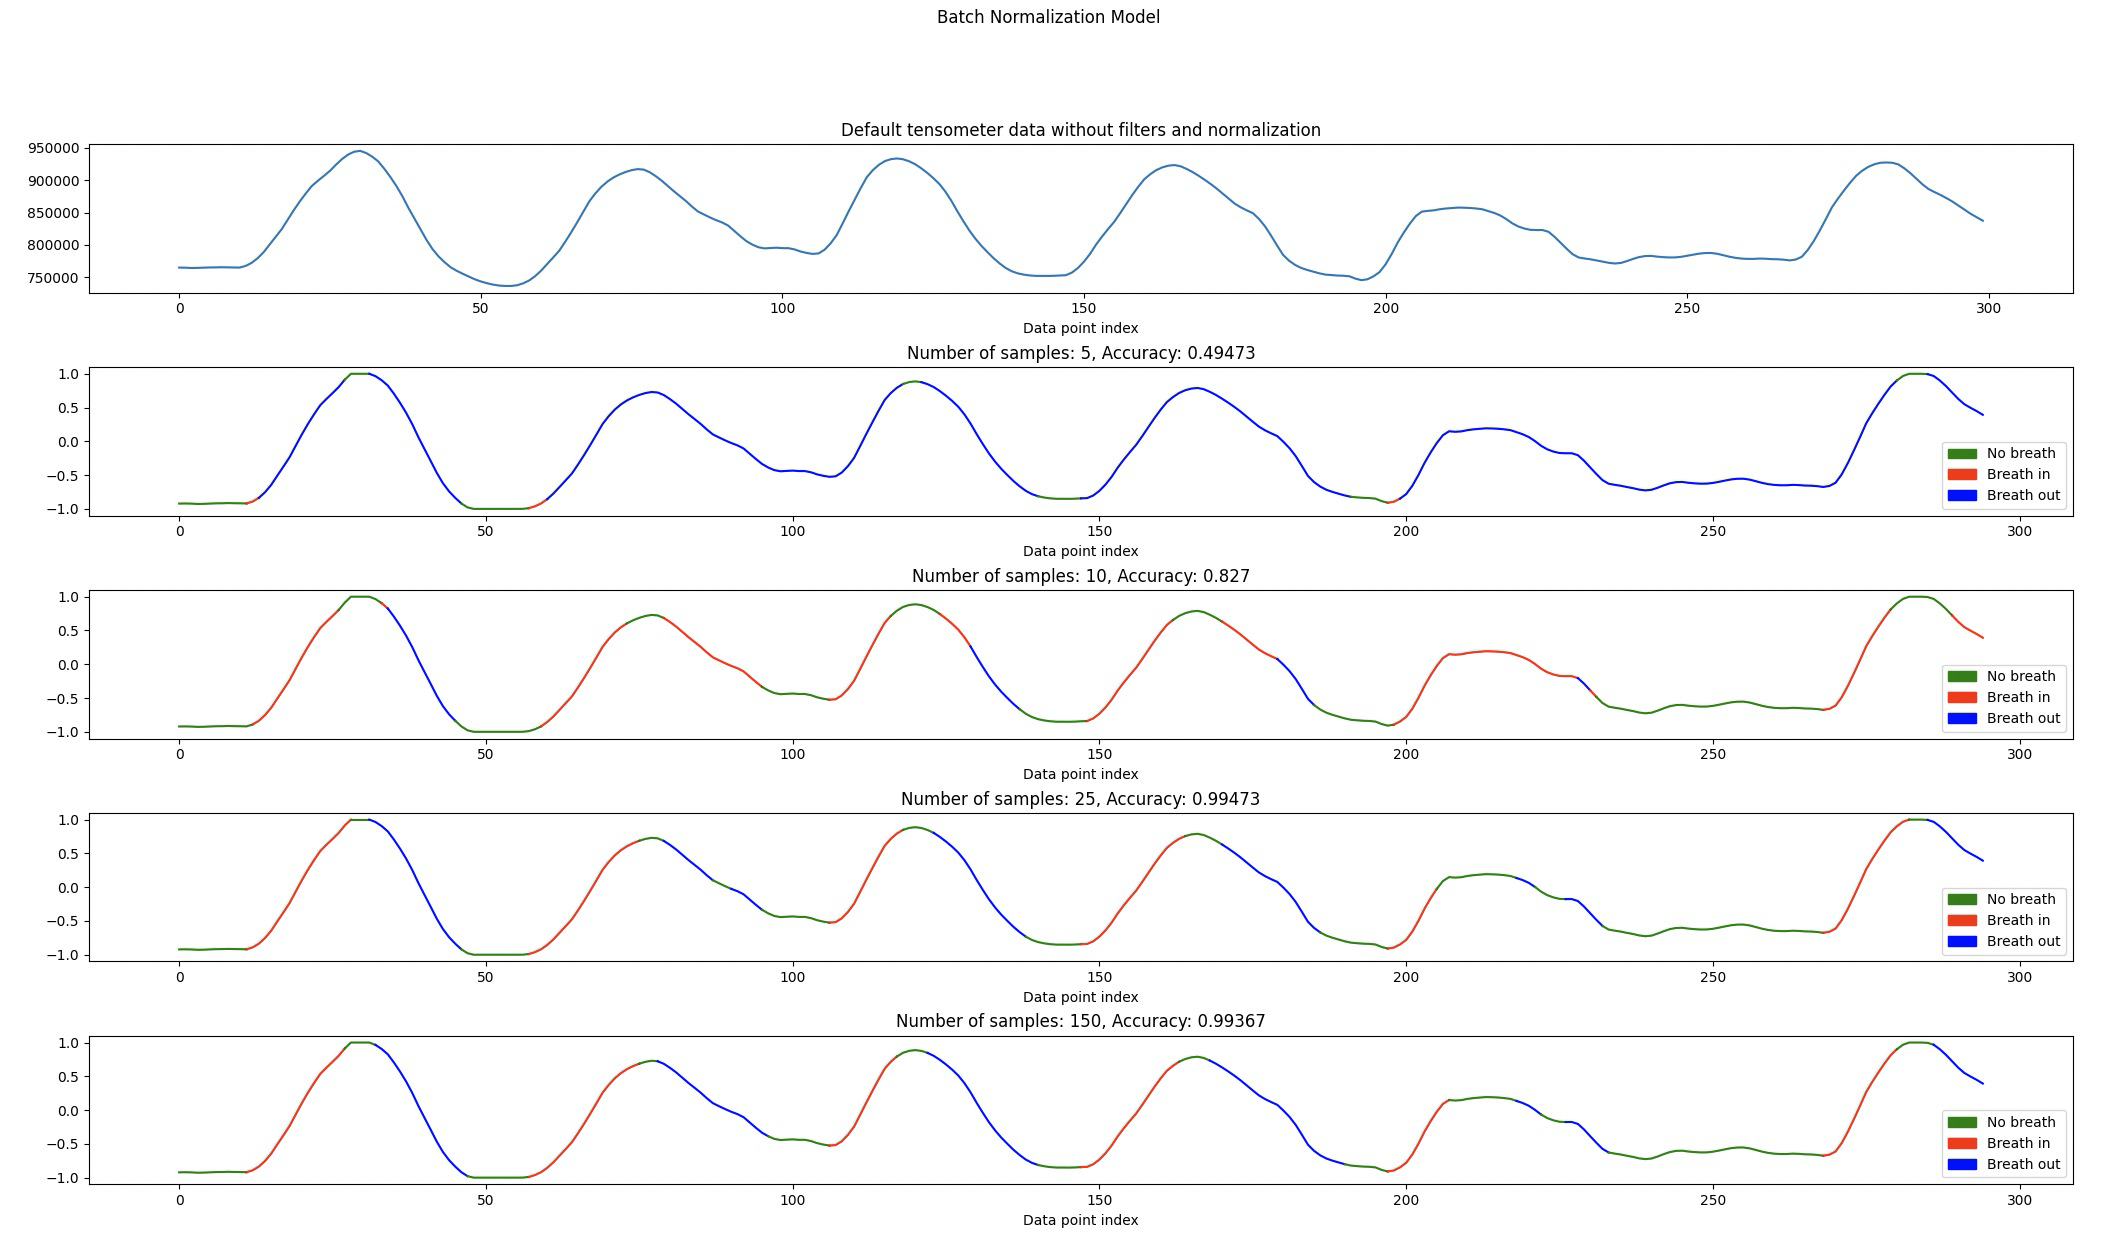
\includegraphics[width=\textwidth]{batch_normalization/skutecznosc.png}
    \caption{Skuteczność modelu Batch Normalization od liczby próbek treningowych dla 300 próbek testowych}
    \label{fig:data_chart7}
\end{figure}

Rys. \ref{fig:data_chart7} przedstawia skuteczność modelu Batch Normalization od liczby próbek treningowych dla 300 próbek testowych. W kolejnych eksperymentach, gdzie liczba próbek wykorzystanych do treningu wynosi odpowiednio 5, 10, 25 i 150 (ilość próbek dla każdego stanu), obserwujemy progresywną poprawę dokładności klasyfikacji od wartości $\sim$0.5 do $\sim$0.99. Wzrost dokładności jest korelowany z zwiększającą się liczbą próbek treningowych, co jest zgodne z powszechnie akceptowanymi założeniami w dziedzinie uczenia maszynowego. Model BatchNormalization wykazuje większą skuteczność względem omawianej wcześniej prostej sieci FeedForward. Wiąże się to z tym, że model BatchNormalization posiada więcej warstw, co pozwala na lepsze wyodrębnienie cech z danych treningowych. Warstwa normalizacji wsadowej (Batch Normalization) analizuje każdą porcję danych, gdy ta napływa. Najpierw normalizuje partię danych za pomocą własnej średniej i odchylenia standardowego, a następnie dostosowuje dane do nowej skali za pomocą dwóch parametrów przeskalowania, które są trenowalne. W efekcie Batch Normalization wykonuje swoisty rodzaj przeskalowywania swoich wejść.


\section{Sieć rekurencyjna}

\subsection{Wstęp}

Sieć rekurencyjna (RNN - Recurrent Neural Network) to rodzaj sztucznej sieci neuronowej, która została zaprojektowana do przetwarzania danych sekwencyjnych lub danych o zmiennej długości, uwzględniając kontekst historyczny. To odróżnia ją od standardowych sieci neuronowych, które traktują dane wejściowe jako niezależne od siebie punkty.

Główną cechą sieci rekurencyjnych jest ich zdolność do pamiętania poprzednich informacji i wykorzystywania ich w przetwarzaniu aktualnych wejść. Składa się z powtarzających się modułów (lub "warstw") zwanych komórkami rekurencyjnymi. Te komórki posiadają wewnętrzny stan, który jest aktualizowany przy każdym kroku czasowym i przechowuje informacje o tym, co sieć "zapamiętała" z poprzednich kroków.

Podczas trenowania sieci rekurencyjnych, algorytm propagacji wstecznej (backpropagation) jest stosowany w celu minimalizacji błędu pomiędzy predykcjami sieci a oczekiwanymi wynikami. W trakcie tego procesu wagi w sieci są dostosowywane tak, aby optymalnie przewidywać dane sekwencyjne.

Istnieje wiele wariantów sieci rekurencyjnych, takich jak:
\begin{itemize}
    \item \textbf{Standardowe RNNs (Vanilla RNNs)}: Prosta forma sieci rekurencyjnej, jednak ma problem z długoterminowymi zależnościami, ponieważ może wystąpić zjawisko zanikającego gradientu (vanishing gradient), co powoduje utratę informacji o odległych zależnościach w sekwencji.
    \item \textbf{Long Short-Term Memory (LSTM)}: Jest to ulepszona wersja RNN, która ma zdolność do przechowywania długoterminowych zależności w danych poprzez specjalne bramki, które decydują, które informacje mają zostać zapamiętane i które mają być zapomniane.
    \item \textbf{Gated Recurrent Unit (GRU)}: Podobne do LSTM, GRU ma mniej bramek, co sprawia, że jest bardziej efektywne obliczeniowo, ale może być mniej elastyczne w przechowywaniu długoterminowych zależności w porównaniu z LSTM.
\end{itemize}

Sieci rekurencyjne są szeroko stosowane w zadaniach przetwarzania języka naturalnego (takich jak tłumaczenie maszynowe, generowanie tekstu), analizy czasowych szeregów, rozpoznawania mowy, generowania muzyki oraz w wielu innych obszarach, gdzie dane posiadają strukturę sekwencyjną. Jednak mają pewne wady, takie jak trudności z równoległym przetwarzaniem, a także problemy z utrzymaniem informacji na długie okresy czasu w standardowych RNNs, które częściowo są rozwiązywane przez bardziej zaawansowane architektury, takie jak LSTM i GRU.

\subsection{Wyniki}

\subsubsection{LSTM}

\begin{figure}[H]
    \centering
    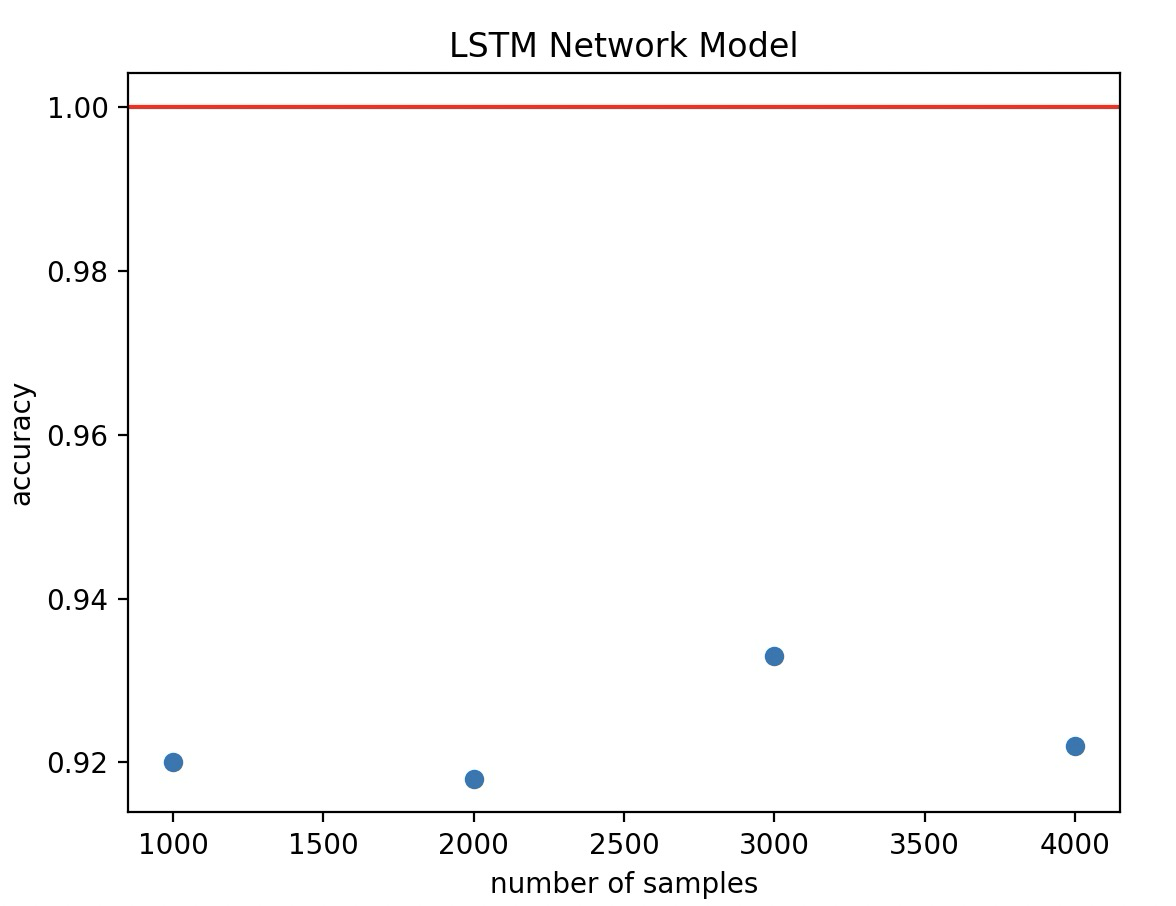
\includegraphics[width=0.75\textwidth]{lstm/dokladnosc.png}
    \caption{Skuteczność modelu LSTM w zależności od liczby próbek treningowych}
    \label{fig:data_chart8}
\end{figure}

Rys. \ref{fig:data_chart8} przedstawia ...

\begin{figure}[H]
    \centering
    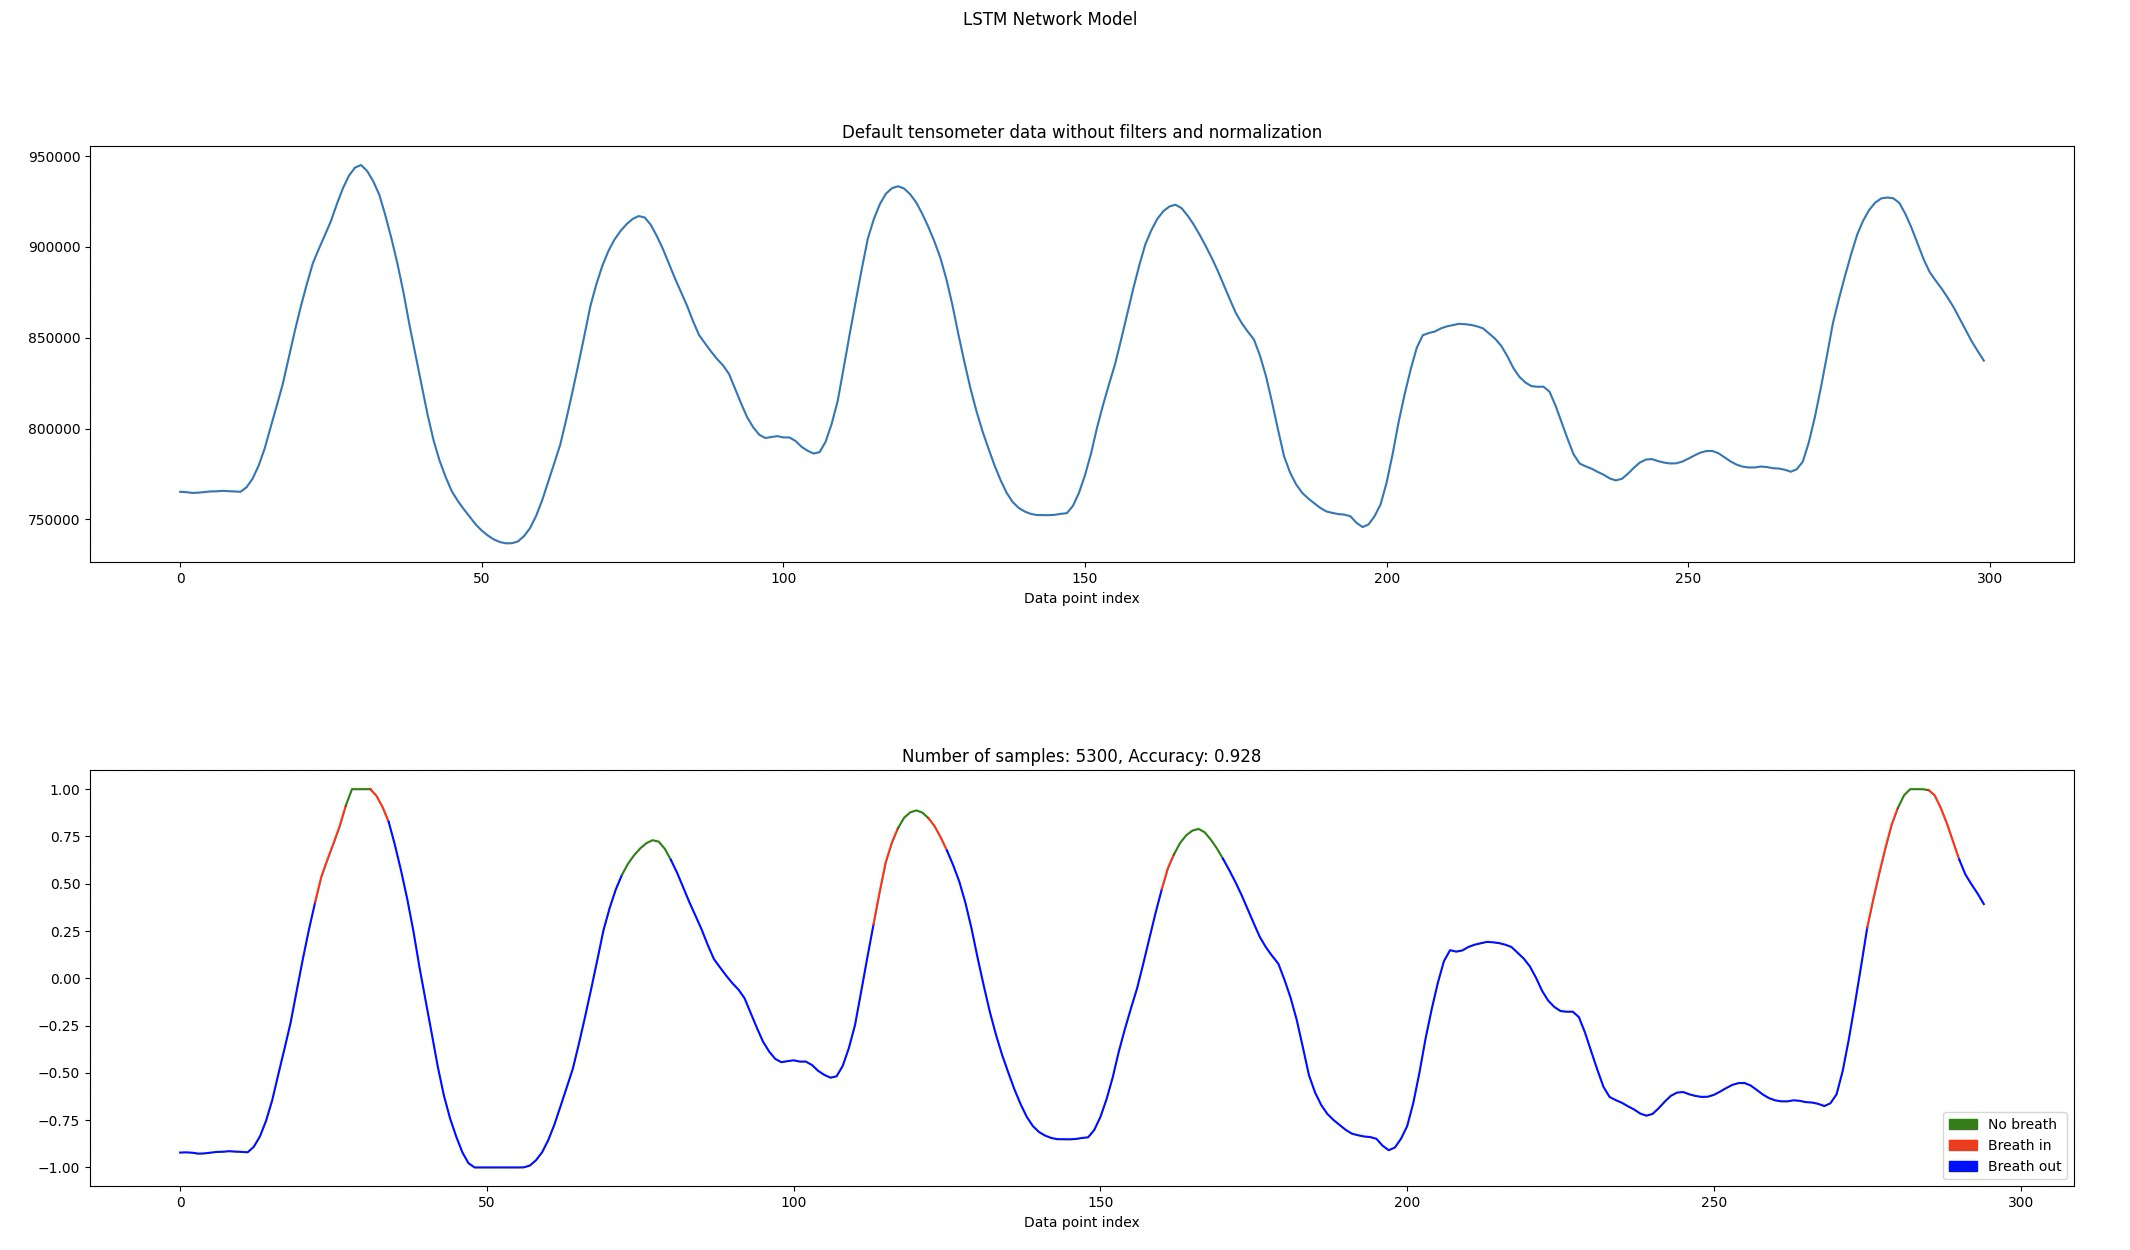
\includegraphics[width=\textwidth]{lstm/skutecznosc.png}
    \caption{Skuteczność modelu LSTM od liczby próbek treningowych dla 300 próbek testowych}
    \label{fig:data_chart9}
\end{figure}

Rys. \ref{fig:data_chart9} przedstawia ...

\subsubsection{GRU}

\begin{figure}[H]
    \centering
    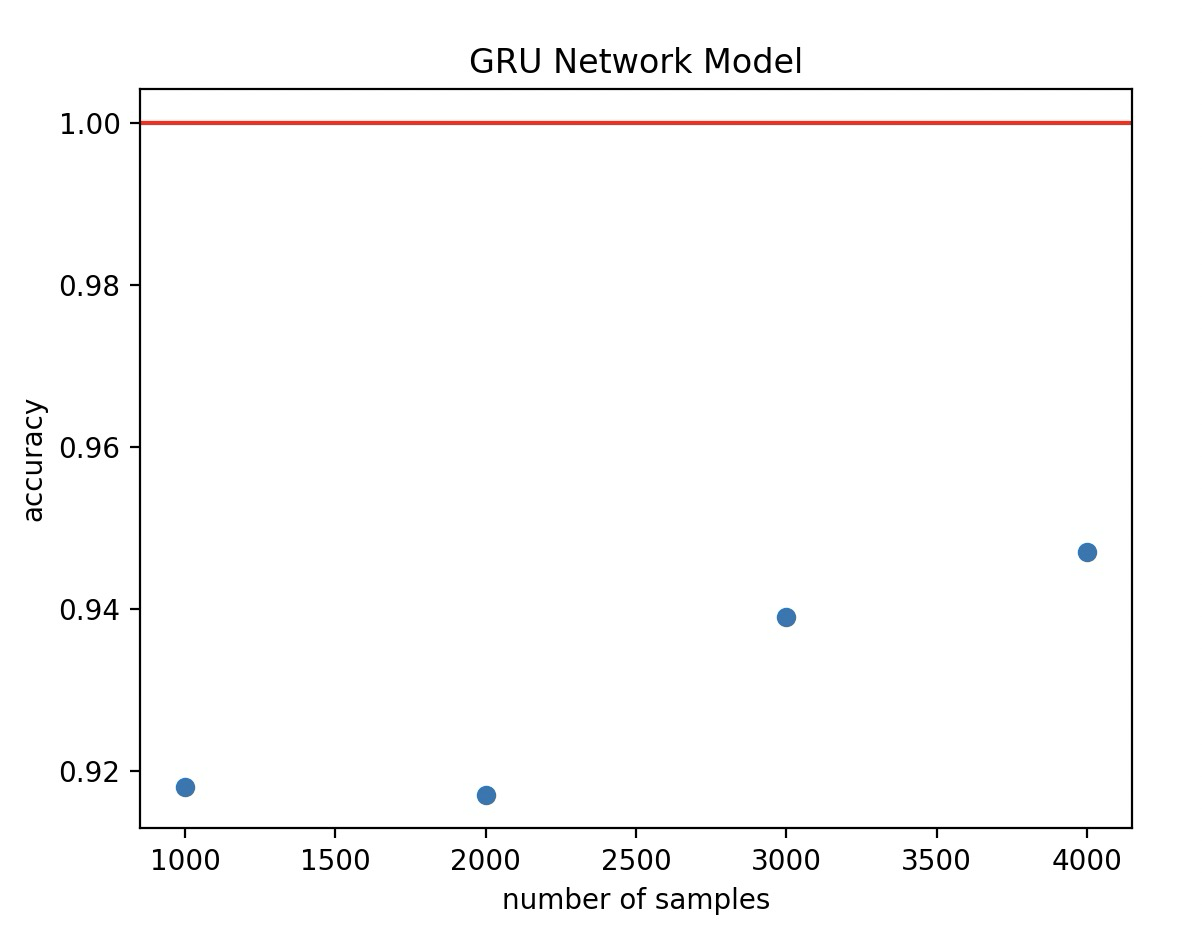
\includegraphics[width=0.75\textwidth]{gru/dokladnosc.png}
    \caption{Skuteczność modelu GRU w zależności od liczby próbek treningowych}
    \label{fig:data_chart10}
\end{figure}

Rys. \ref{fig:data_chart10} przedstawia ...

\begin{figure}[H]
    \centering
    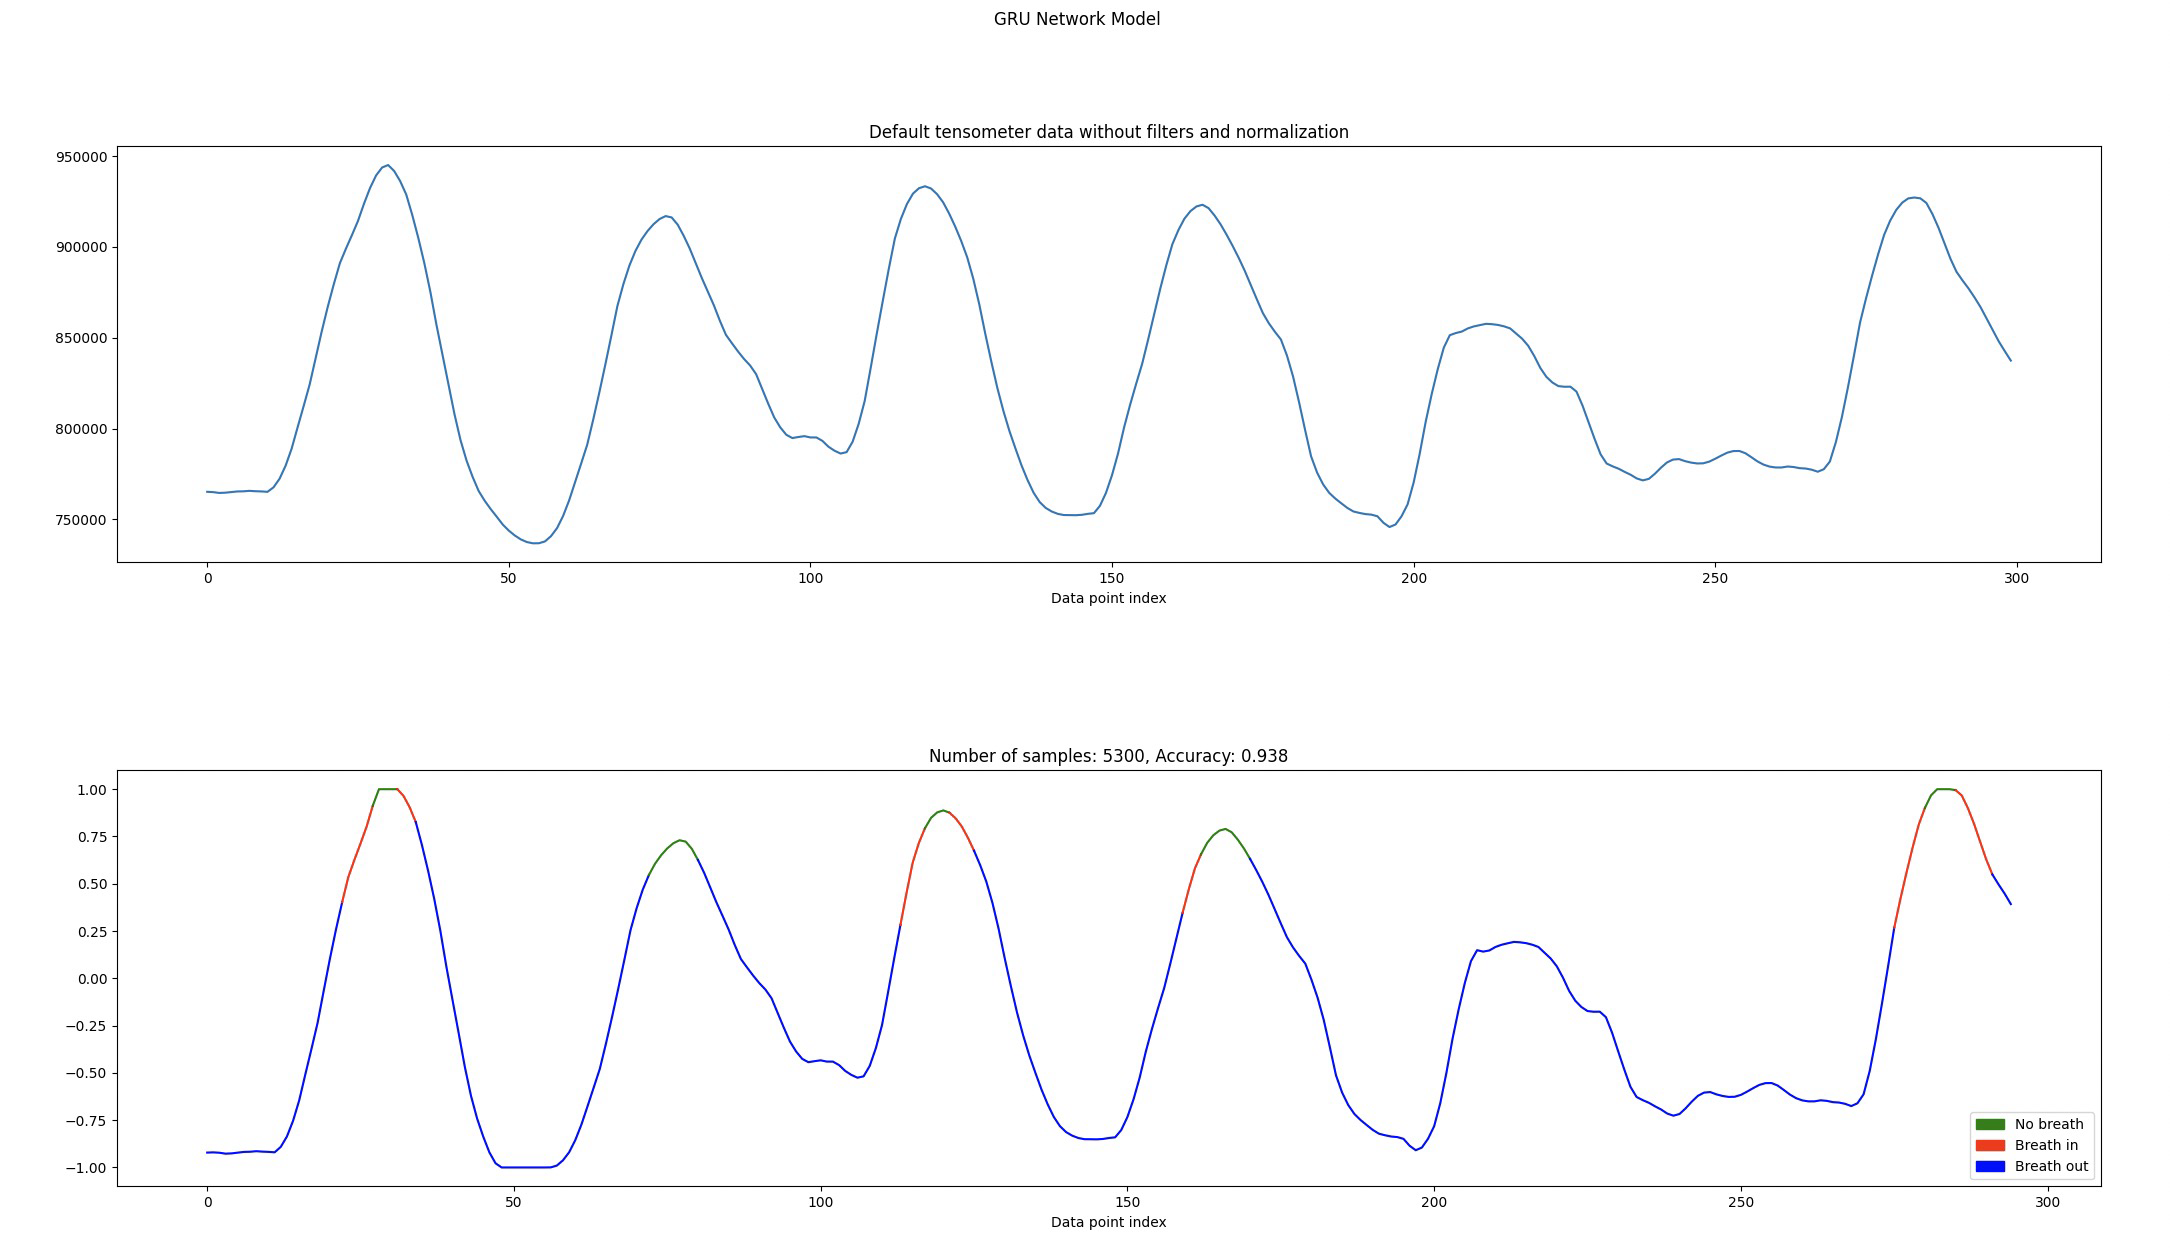
\includegraphics[width=\textwidth]{gru/skutecznosc.png}
    \caption{Skuteczność modelu GRU od liczby próbek treningowych dla 300 próbek testowych}
    \label{fig:data_chart11}
\end{figure}

Rys. \ref{fig:data_chart11} przedstawia ...

\section{Sieć konwolucyjna}

\subsection{Wstęp}

Sieci konwolucyjne 1D (Convolutional Neural Networks - CNNs) są odmianą architektury sieci neuronowej, które specjalizują się w przetwarzaniu danych sekwencyjnych, takich jak sygnały czasowe, szeregi czasowe, sekwencje tekstowe itp. Podobnie jak w przypadku klasycznych sieci konwolucyjnych dla danych obrazowych (2D), sieci 1D wykorzystują operacje konwolucji do wyodrębniania cech.

Główne elementy sieci konwolucyjnych 1D to:

\begin{enumerate}

\item \textbf{Warstwy konwolucyjne}: Składają się z zestawu filtrów (jąder konwolucyjnych), które przesuwają się po sekwencji wejściowej w celu wydobycia lokalnych cech. Filtry te są stosowane wzdłuż wymiaru czasowego danych (np. wzdłuż sekwencji tekstu).

\item \textbf{Warstwy poolingowe}: Po warstwach konwolucyjnych często następują warstwy poolingowe, które zmniejszają rozmiar przestrzeni cech, zachowując istotne informacje. Najczęściej używane są warstwy MaxPooling, które wybierają największą wartość z określonych fragmentów danych.

\item \textbf{Warstwy aktywacji}: Po każdej operacji konwolucji lub pooling, stosuje się funkcje aktywacji, takie jak ReLU (Rectified Linear Unit) w celu wprowadzenia nieliniowości i ułatwienia uczenia się modelu.

\item \textbf{Warstwy w pełni połączone (fully connected layers)}: Po przetworzeniu przez warstwy konwolucyjne i poolingowe, w ostatniej części sieci 1D umieszcza się warstwy w pełni połączone, które agregują cechy i dokonują końcowego przetwarzania w celu klasyfikacji lub prognozowania.

\end{enumerate}
Zastosowania sieci konwolucyjnych 1D obejmują:

\begin{itemize}

\item Analizę szeregów czasowych: Takie jak prognozowanie cen akcji, przetwarzanie sygnałów biomedycznych czy też rozpoznawanie gestów w sygnałach czasowych.
\item Przetwarzanie języka naturalnego: Wykrywanie emocji w zdaniach, klasyfikacja tekstów czy też generowanie opisów.
\item Sieci konwolucyjne 1D stanowią skuteczną architekturę do przetwarzania danych sekwencyjnych, ponieważ potrafią wydobywać ważne lokalne cechy i wzorce, co czyni je przydatnymi w wielu dziedzinach analizy danych.

\end{itemize}

\subsection{Wyniki}

\begin{figure}[H]
    \centering
    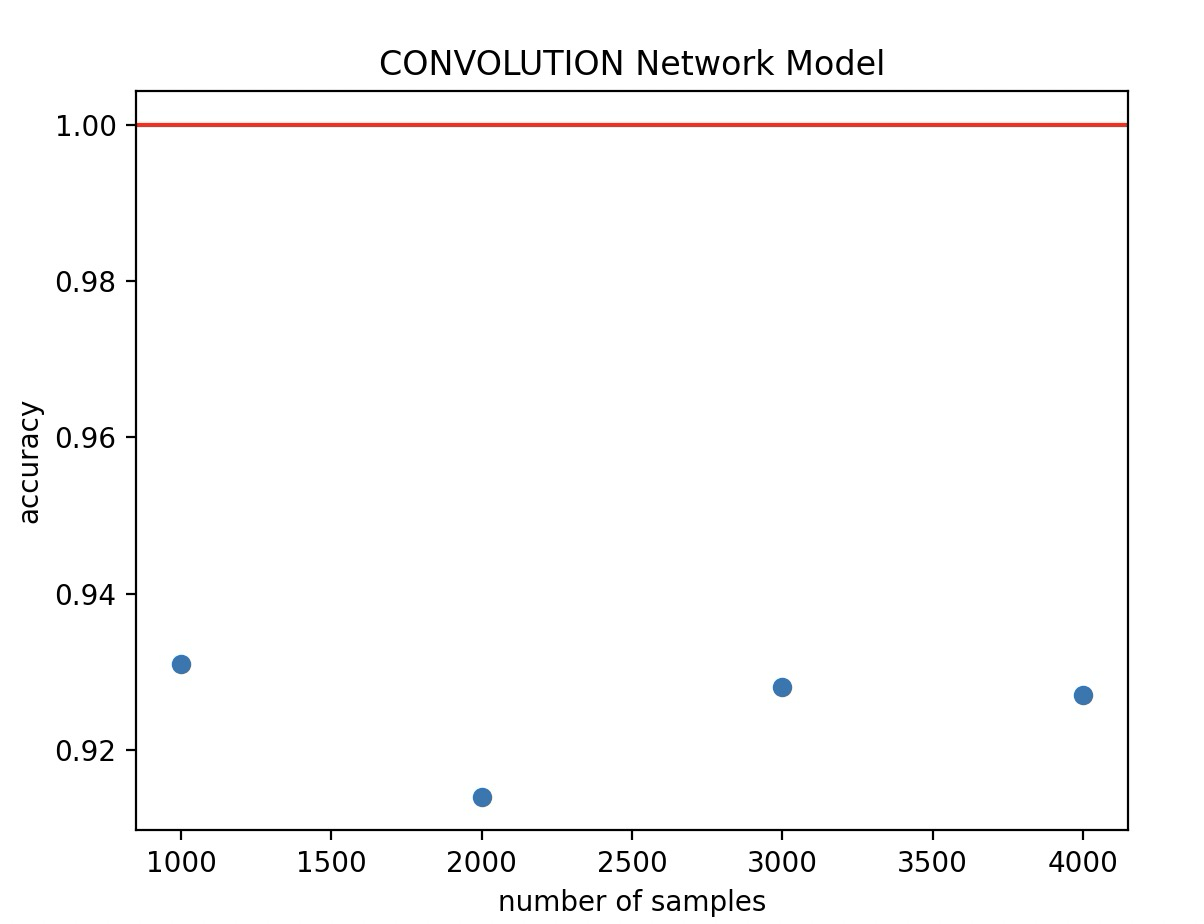
\includegraphics[width=0.75\textwidth]{rek/dokladnosc.png}
    \caption{Skuteczność modelu sieci konwolucyjnej w zależności od liczby próbek treningowych}
    \label{fig:data_chart12}
\end{figure}

Rys. \ref{fig:data_chart12} przedstawia ...

\begin{figure}[H]
    \centering
    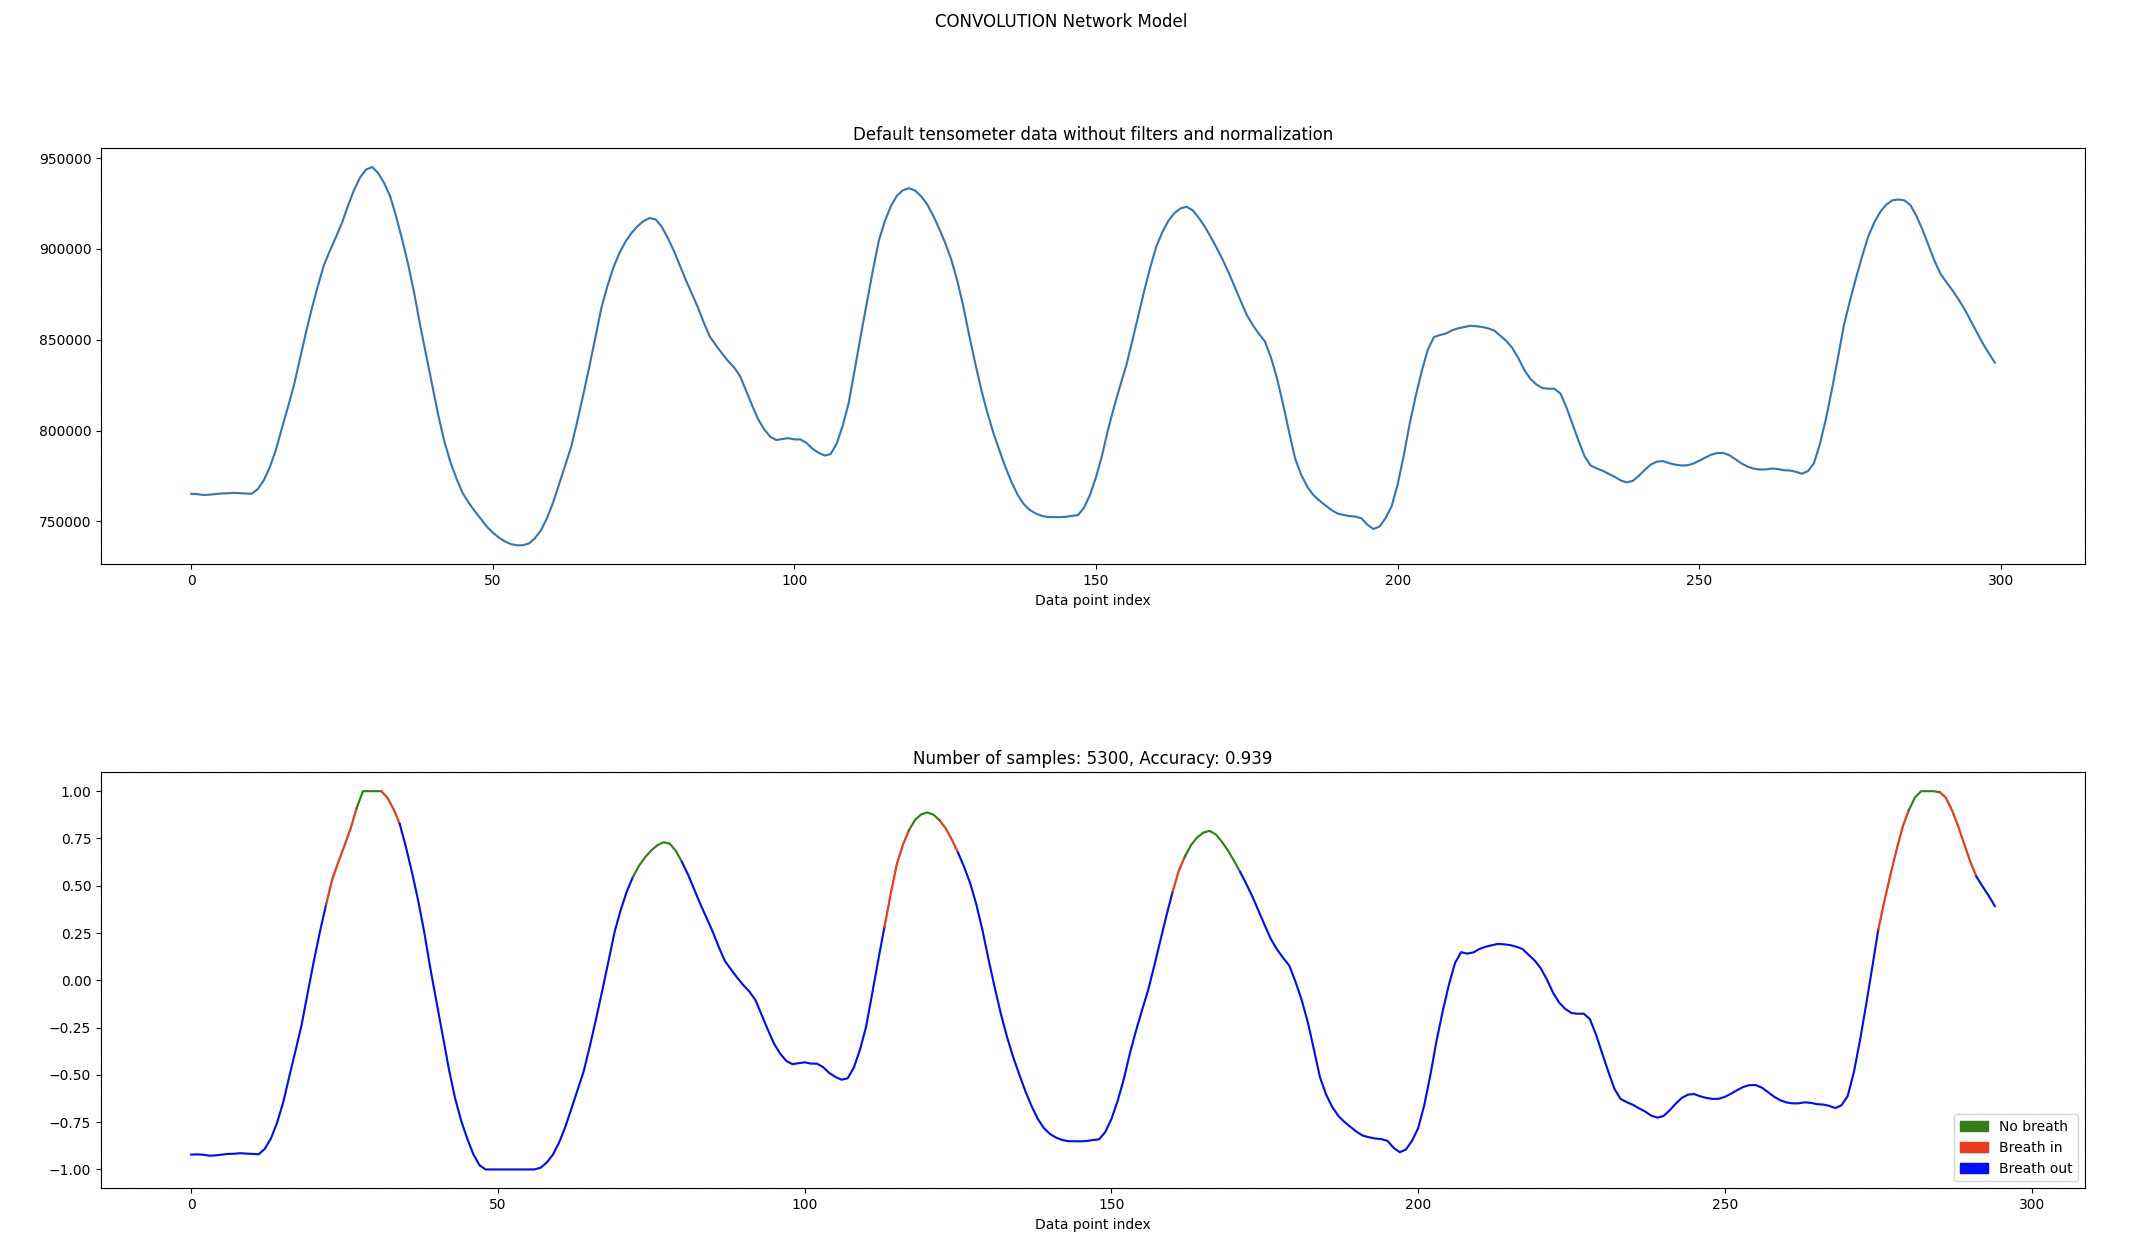
\includegraphics[width=\textwidth]{rek/skutecznosc.png}
    \caption{Skuteczność modelu sieci konwolucyjnej od liczby próbek treningowych dla 300 próbek testowych}
    \label{fig:data_chart13}
\end{figure}

Rys. \ref{fig:data_chart13} przedstawia ...

\end{document}